% Author: Max Melching, 2025
% Heavily inspired by Figure 9-10 from Thornton, Marion - Classical Dynamics of Particles and Systems
\documentclass[border=3pt,tikz]{standalone}


\usepackage{tikz}
\usepackage{pgfplots} % for the axis environment
\usepackage[outline]{contour}
\usepackage{xcolor}
\usepackage{newtxmath}  % Use Times in math mode
\usepackage{tgpagella}  % Use Pagella in text


\colorlet{mydarkred}{red!70!black}
\colorlet{mydarkgreen}{green!50!black}
\colorlet{myblue}{blue!80!black}


\usetikzlibrary{arrows.meta, calc, decorations.markings, math}


\tikzset{
    >={Stealth[inset=0,angle'=27]},
    lab velocity/.style={
        ->,
        thick,
    },
    com velocity/.style={
        ->,
        thick,
        mydarkgreen,
    },
    angle/.style={
        ->,
        semithick,
        % scale=0.5,  % Trying to make arrow tip smaller
        mydarkred,
        % myblue,
    },
    mass/.style={
        % mydarkred,
        myblue,
        fill,
    },
}



\begin{document}


\def\mone{3}
\def\mtwo{5}
\def\V{2}


\begin{tikzpicture}
	\tikzmath{
        \M=\mone+\mtwo;
        \vone=\M/\mone*\V;
        \uoneprime=\vone-\V;
        \utwoprime=-\V;
	}

    \coordinate (m1) at (0,0);
    \coordinate (m2) at (8,0);
    \coordinate (V) at (\V, 0);
    \coordinate (v1) at (\vone, 0);
    \coordinate (u1') at (\uoneprime, 0);
    \coordinate (u2') at (\utwoprime, 0);
    

    \draw[mass] (m1) circle(0.04) node[left] {$m_1$};
    \draw[mass] (m2) circle(0.04) node[right] {$m_2$};

    \draw[lab velocity] (m1) -- ++(v1) node[pos=0.8, above] {$\vec{v}_1$};
    \node[above] at (m2) {$\vec{v}_2 = 0$};
    
    % \draw[com velocity] (m1) --++ (V) node[pos=0.5, below] {$\vec{V}$};
    % \draw[com velocity] (m1) --++ (u1') node[pos=0.75, below] {$\vec{u}'_1$};
    % \draw[com velocity] (m2) --++ (u2') node[pos=0.5, below] {$\vec{u}'_2$};
    
    \draw[com velocity] (m1) ++ (\uoneprime,-0.5) --++ (V) node[pos=0.5, below] {$\vec{V}$};  % Shift so that u'_1 is more visible
    \draw[com velocity] (m1) --++ (u1') node[pos=0.5, below] {$\vec{u}'_1$};
    \draw[com velocity] (m2) --++ (u2') node[pos=0.5, below] {$\vec{u}'_2$};

\end{tikzpicture}



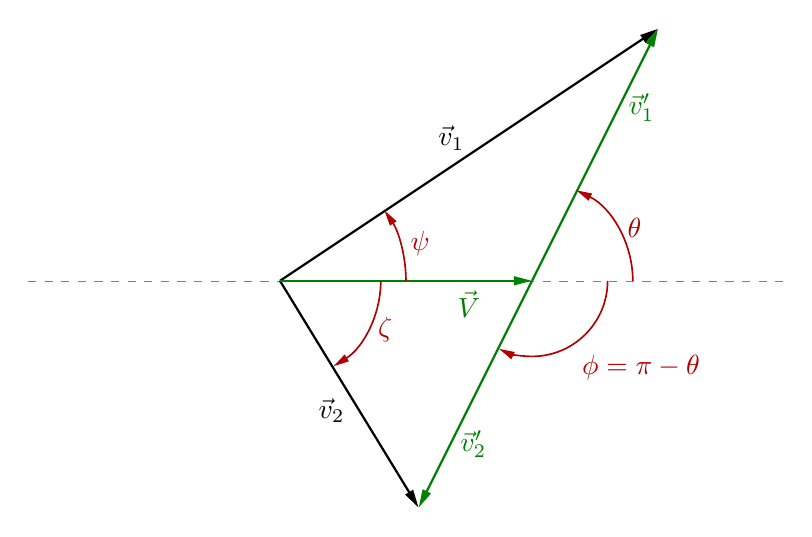
\begin{tikzpicture}[scale=1.6]
    \coordinate (O) at (0, 0);
    \coordinate (V) at (2, 0);
    \coordinate (v1) at (3, 2);
    % \coordinate (v2) at (1, -2);
    \coordinate (v2) at ($(V) - 0.9*(v1)+0.9*(V)$);  % Is not independent of V, v1


    \draw[help lines, dashed] ($-1*(V)$) -- ($2*(V)$);

    % \draw[velocity] (O) -- (V) node[pos=0.75, below] {$V$};
    % \draw[velocity] (O) -- (v1) node[midway, above left=-2] {$v_1$};
    % \draw[velocity] (O) -- (v2) node[midway, below left=-2] {$v_2$};
    
    % \draw[help lines] (v1) -- (v2) node {};
    

    \draw[lab velocity] (O) -- (v1) node[midway, above left=-2] {$\vec{v}_1$};
    \draw[lab velocity] (O) -- (v2) node[midway, below left=-2] {$\vec{v}_2$};
    \draw[com velocity] (O) -- (V) node[pos=0.75, below] {$\vec{V}$};
    \draw[com velocity] (V) -- (v1) node[pos=0.75, below right=-3] {$\vec{v}'_1$};
    \draw[com velocity] (V) -- (v2) node[pos=0.65, below right=-3] {$\vec{v}'_2$};


    \def\arcrad{0.8}
    \def\rtheta{64}
    \draw[angle] (V) ++ (\arcrad,0) arc(0:\rtheta:\arcrad) node[midway, right] {$\theta$};
    % \def\arcrad{1}
    \def\arcrad{0.6}
    \def\rthetatwo{\rtheta-180}
    \draw[angle] (V) ++ (\arcrad,0) arc(0:\rthetatwo:\arcrad) node[midway, below right] {$\phi = \pi - \theta$};
    \def\arcrad{1}
    \def\rpsi{34}
    \draw[angle] (O) ++ (\arcrad,0) arc(0:\rpsi:\arcrad) node[midway, right] {$\psi$};
    \def\arcrad{0.8}
    \def\rzeta{-58}
    \draw[angle] (O) ++ (\arcrad,0) arc(0:\rzeta:\arcrad) node[midway, right] {$\zeta$};

\end{tikzpicture}


\end{document}